\documentclass[12pt,addpoints]{uofmexamNoHeader}

\usepackage{enumitem}

%\makeatletter
%%%%%%%%%%%%%%%%%
\PassOptionsToPackage{force}{filehook}
\usepackage{tikz}
%\usetikzlibrary{shapes}
\usetikzlibrary{plotmarks}
\usetikzlibrary{positioning}% To get more advances positioning options
\usetikzlibrary{arrows}
\usetikzlibrary{patterns}

\usetikzlibrary{calc}
\usepackage{dsfont}
\usetikzlibrary{calc}
\tikzset{smalldot/.style={circle,draw=black,fill=black,inner sep = 1pt}}

\usetikzlibrary{calc}
\tikzset{smalldot/.style={circle,draw=black,fill=black,inner sep = 1.5pt}}
\tikzset{opendot/.style={circle,draw=black,fill=white,inner sep = 1.5pt}}

\usetikzlibrary{shapes,arrows}
\usetikzlibrary{positioning}
\tikzstyle{cloud} = [draw, ellipse,fill=red!20, node distance=0.87cm,
minimum height=2em]
\tikzstyle{line} = [draw, -latex']
\usetikzlibrary{shapes.symbols,shapes.callouts,patterns}
\usetikzlibrary{calc,fit}
\usetikzlibrary{backgrounds}

\def\IC{\mathbb{C}}
\def\IF{\mathbb{F}}
\def\II{\mathbb{I}}
\def\IN{\mathbb{N}}
\def\IR{\mathbb{R}}
\def\IZ{\mathbb{Z}}

\def\b0{\mathbf{0}}
\def\bb{\mathbf{b}}
\def\be{\mathbf{e}}
\def\bi{\mathbf{i}}
\def\bj{\mathbf{j}}
\def\bk{\mathbf{k}}
\def\bu{\mathbf{u}}
\def\bv{\mathbf{v}}
\def\bw{\mathbf{w}}
\def\bx{\mathbf{x}}
\def\by{\mathbf{y}}
\def\bz{\mathbf{z}}

\def\B{\mathcal{B}}
\def\C{\mathcal{C}}
\def\E{\mathcal{E}}
\def\L{\mathcal{L}}
\def\M{\mathcal{M}}
\def\N{\mathcal{N}}

\def\ker{\ensuremath{\text{ker}}}


\newtheorem{theorem}{Theorem}
\newtheorem{definition}[theorem]{Definition}

\newcommand{\dist}[1]{\mathsf{dist}[#1]}
\newcommand{\prev}[1]{\mathsf{prev}[#1]}
\def\alt{\text{\tt alt}\ }
\def\length{\text{\tt length}}


\examinfo{%
	type={ASSIGNMENT 8},	% Optional; leave blank or do not specify to omit.
	coursenumber={MATH 2740},	% include section, unless this is a multisection exam.
	%crn={CRN},	% Optional; leave blank or do not specify to omit.
	%examiner={Examiner},	% Optional; leave blank or do not specify to omit
	duration={1 week},
	date={Due 11 October},
	time={12:00},
	crowdmark=duplex,	% single sided is the default (no =duplex); use crowdmark=duplex for two-sided.
	}

% uncomment \printanswers for a solution key
%\printanswers

\pointsinmargin
\bracketedpoints

\geometry{letterpaper,bottom=0.5in}	% legalpaper is the default.

%%%%%%%%%%%%%%%%%%%%%%%%%%%%%%%%%%%%%%%%%%%%%
\begin{document}

\begin{center}
	\large
	\textbf{AARMS 2023 Summer School\\20--30 August 2023\\Stochastic models problem set}\\[0.5cm]
\end{center}

\begin{questions}

%%%%%%%%%%%%%%%%%%%%%%%%%%%%%%%%%%%%%%%%%%%%%
\question[10]
Consider the Kermack-McKendrick SIR \emph{epidemic} model
\begin{center}
    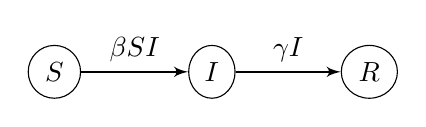
\begin{tikzpicture}[auto,
        cloud/.style={minimum width={width("-12")+2pt},
            draw, ellipse},
        connected/.style={dotted,-}]
        %% Vertices
        \node [cloud] at (0,0) (S) {$S$};
        \node [cloud] at (2,0) (I){$I$};
        \node [cloud] at (4,0) (R){$R$};
        %% Arcs
        \path [line, thick] (S) to node [midway, above] (TextNode) {$\beta SI$} (I);
        \path [line, thick] (I) to node [midway, above] (TextNode) {$\gamma I$} (R);
    \end{tikzpicture}
\end{center}
Convert the Kermack-McKendrick SIR model to a continuous-time Markov chain model.
\begin{parts}
    \part List the state transition and their weights.
    \part Write the Gillespie algorithm you would use to simulate the chain.
    \part Write some code to run several simulations of the chain using {\tt adaptivetau} or {\tt GillespieSSA2}.
    Plot the solution in three different graphs.
    \part For good measure, plot the average prevalence as well as the prevalence in the corresponding ODE.
    (For the former, you will probably need to interpolate solutions.)
\end{parts}

\begin{solution}
\end{solution}

\vfill

\question[10]
Consider the \emph{endemic} SIR model with demography
\begin{center}
    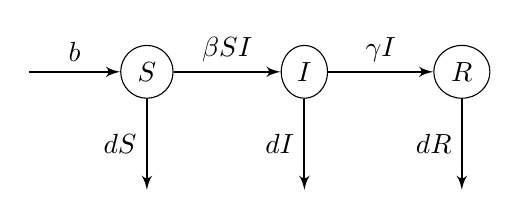
\begin{tikzpicture}[auto,
        cloud/.style={minimum width={width("-12")+2pt},
            draw, ellipse},
        connected/.style={dotted,-}]
        %% Vertices
        \node [cloud] at (0,0) (S) {$S$};
        \node [cloud] at (2,0) (I){$I$};
        \node [cloud] at (4,0) (R){$R$};
        %% Arcs
        \path [line, thick] (-1.5,0) to node [midway, above] (TextNode) {$b$} (S);
        \path [line, thick] (S) to node [midway, above] (TextNode) {$\beta SI$} (I);
        \path [line, thick] (S) to node [midway, left] (TextNode) {$dS$} (0,-1.5);
        \path [line, thick] (I) to node [midway, above] (TextNode) {$\gamma I$} (R);
        \path [line, thick] (I) to node [midway, left] (TextNode) {$dI$} (2,-1.5);
        \path [line, thick] (R) to node [midway, left] (TextNode) {$dR$} (4,-1.5);
    \end{tikzpicture}
\end{center}
Convert the SIR endemic model with demography to a continuous-time Markov chain model.
\begin{parts}
    \part List the state transition and their weights.
    \part Write the Gillespie algorithm you would use to simulate the chain.
    \part Write some code to run several simulations of the chain using {\tt adaptivetau} or {\tt GillespieSSA2}. 
    Plot the solution in three different graphs.
    \part For good measure, plot the average prevalence as well as the prevalence in the corresponding ODE.
    (For the former, you will probably need to interpolate solutions.)
\end{parts}

\vfill

\newpage
\question[10]
Consider the \emph{epidemic} SLIAR model
\begin{center}
    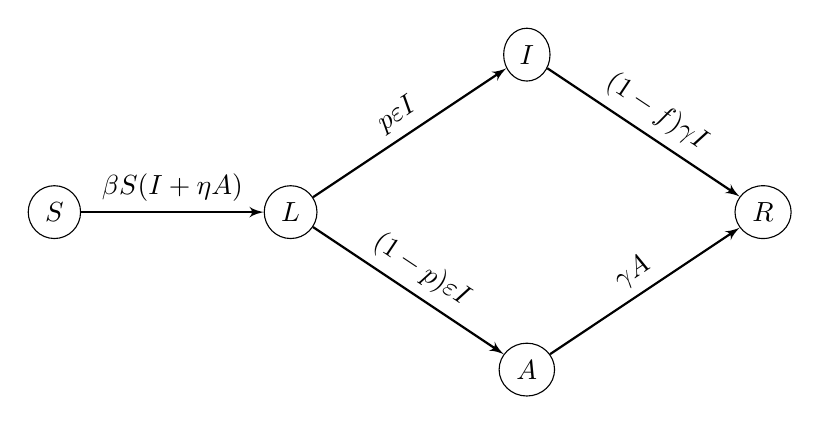
\begin{tikzpicture}[auto,
        cloud/.style={minimum width={width("-12")+2pt},
            draw, ellipse},
        connected/.style={dotted,-}]
        %% Vertices
        \node [cloud] at (0,0) (S) {$S$};
        \node [cloud] at (3,0) (L){$L$};
        \node [cloud] at (6,2) (I){$I$};
        \node [cloud] at (6,-2) (A){$A$};
        \node [cloud] at (9,0) (R){$R$};
        %% Arcs
        \path [line, thick] (S) to node [midway, above] (TextNode) {$\beta S(I+\eta A)$} (L);
        \path [line, thick, sloped] (L) to node [midway, above] (TextNode) {$p\varepsilon I$} (I);
        \path [line, thick, sloped] (L) to node [midway, above] (TextNode) {$(1-p)\varepsilon I$} (A);
        \path [line, thick, sloped] (I) to node [midway, above] (TextNode) {$(1-f)\gamma I$} (R);
        \path [line, thick, sloped] (A) to node [midway, above] (TextNode) {$\gamma A$} (R);
    \end{tikzpicture}
\end{center}
Convert the epidemic SLIAR model to a continuous-time Markov chain model.
\begin{parts}
    \part List the state transition and their weights.
    \part Write some code to run several simulations of the chain using {\tt GillespieSSA2}.
    \part For good measure, plot the average solution as well as the corresponding ODE.
    (For the former, you will probably need to interpolate the solutions.)
    \part Use the {\tt log\_firings = TRUE} option of {\tt ssa} in {\tt GillespieSSA2} to log events and plot incidence, and decompose incidence in terms of symptomatic and asymptomatic infections.
    \part (Bonus) Plot the quantities in (d) as epi graphs.
    \part (Bonus) Reinterpreting $I$ as detected infections and $A$ as undetected infections, discuss making $p$, the proportion of detected infections, a function of .. something. (It could be time, prevalence, etc.)
\end{parts}




\end{questions}
\end{document}